\begin{document}

\title {\ZHH \huge HTML5之WebSocket}
\author {\small gaccob}
\date {\small 2013 年 6 月 14 日}
\maketitle

\section {\ZHH 什么是WebSocket} {
    {WebSocket是HTML5提出的一个\textcolor{blue}{协议规范}, 参考\href{http://tools.ietf.org//rfc6455}{rfc6455}. 不过目前还都是在草案, 没有成为标准, 毕竟HTML5还在路上.} \par

    {WebSocket约定了一个通信的规范, 通过一个握手的机制, 客户端(浏览器)和服务器(WebServer)之间能建立一个类似tcp的连接, 从而方便c-s之间的通信.}\par
    {在WebSocket出现之前, web交互一般是基于HTTP协议的短连接或者长连接. 短连接的过程大概有下面几个步骤: 建立tcp连->浏览器发出HTTP请求->WebServer应答->断开tcp连接.}\par

    {优点是简洁明了, 缺点也很明显, 每一次的交互中, 建立和断开tcp连接带来了比较大的开销, 而且HTTP协议头比较长, 也会带来带宽的浪费.}\par

    {通过设置HTTP头中的keep-alive域可以实现HTTP长连接, 避免了建立和断开连接的开销, 但是HTTP协议头的问题仍然无法解决.}\par

    {除此之外, WebServer主动向浏览器推送数据的处理会比较麻烦, 要么是浏览器发起轮询(毫无疑问, 这是一个低效的方式), 或者利用\href{http://zh.wikipedia.org/wiki/Comet\_(web\%E6\%8A\%80\%E6\%9C\%AF)}{comet技术}, 比较复杂, 而且这已经不是在层面上解决问题了.}\par

    {而WebSocket的出现, 解决了上面描述的问题.}\par
}

\section {\ZHH WebSocket握手协议} {
    {WebSocket是一种全新的协议, 不属于HTTP无状态协议, 协议名为"ws", 这意味着一个WebSocket连接地址会是这样的写法:ws://**.}\par

    {WebSocket协议本质上是一个基于tcp的协议. 建立连接需要握手, 客户端(浏览器)首先向服务器(WebServer)发起一条特殊的http请求, WebServer解析后生成应答到浏览器, 这样子一个WebSocket连接就建立了, 直到某一方关闭连接.}\par

    {由于是草案的原因, 前前后后就出现了多个版本的握手协议, 分情况说明一下.}\par

    {\textcolor{blue}{基于flash的握手协议},  使用场景是IE的多数版本, 因为IE的多数版本不都不支持WebSocket协议, 以及FF、CHROME等浏览器的低版本, 还没有原生的支持WebSocket. 此处, server唯一要做的, 就是准备一个WebSocket-Location域给client, 没有加密, 可靠性很差.}\par

\begin{lstlisting}[language=bash]
#客户端请求:
GET /ls HTTP/1.1
Upgrade: WebSocket
Connection: Upgrade
Host: www.xx.com
Origin: http://www.xx.com

#服务器返回:
HTTP/1.1 101 Web Socket Protocol Handshake
Upgrade: WebSocket
Connection: Upgrade
WebSocket-Origin: http://www.xx.com
WebSocket-Location: ws://www.xx.com/ls
\end{lstlisting}

    {\textcolor{blue}{基于md5加密方式的握手协议}}\par

\begin{lstlisting}[language=bash]
# 客户端请求:
GET /demo HTTP/1.1
Host: example.com
Connection: Upgrade
Sec-WebSocket-Key2: **
Upgrade: WebSocket
Sec-WebSocket-Key1: **
Origin: http://example.com
[8-byte security key]

# 服务端返回:
HTTP/1.1 101 WebSocket Protocol Handshake
Upgrade: WebSocket
Connection: Upgrade
WebSocket-Origin: http://example.com
WebSocket-Location: ws://example.com/demo
[16-byte hash response]
\end{lstlisting}

    {其中 Sec-WebSocket-Key1, Sec-WebSocket-Key2 和 [8-byte security key] 这几个头信息是web server用来生成应答信息的来源, 依据 draft-hixie-thewebsocketprotocol-76 草案的定义, web server基于以下的算法来产生正确的应答信息:}\par

    \begin{enumerate}
        \item{逐个字符读取 Sec-WebSocket-Key1 头信息中的值, 将数值型字符连接到一起放到一个临时字符串里, 同时统计所有空格的数量.}\par
        \item{将在第(1)步里生成的数字字符串转换成一个整型数字, 然后除以第(1)步里统计出来的空格数量, 将得到的浮点数转换成整数型.}\par
        \item{将第(2)步里生成的整型值转换为符合网络传输的网络字节数组.}\par
        \item{对 Sec-WebSocket-Key2 头信息同样进行第(1)到第(3)步的操作, 得到另外一个网络字节数组.}\par
        \item{将 [8-byte security key] 和在第(3)、(4)步里生成的网络字节数组合并成一个16字节的数组. }\par
        \item{对第(5)步生成的字节数组使用MD5算法生成一个哈希值, 这个哈希值就作为安全密钥返回给客户端, 以表明服务器端获取了客户端的请求, 同意创建WebSocket连接. }\par
    \end{enumerate}

    {\textcolor{blue}{基于sha加密方式的握手协议},  也是目前见的最多的一种方式, 这里的版本号目前是需要13以上的版本.}\par

\begin{lstlisting}[language=bash]
# 客户端请求:
GET /ls HTTP/1.1
Upgrade: websocket
Connection: Upgrade
Host: www.xx.com
Sec-WebSocket-Origin: http://www.xx.com
Sec-WebSocket-Key: 2SCVXUeP9cTjV+0mWB8J6A==
Sec-WebSocket-Version: 13

# 服务器返回:
HTTP/1.1 101 Switching Protocols
Upgrade: websocket
Connection: Upgrade
Sec-WebSocket-Accept: mLDKNeBNWz6T9SxU+o0Fy/HgeSw=
\end{lstlisting}

    {它的原理, 是把客户端上报的key拼上一段GUID “258EAFA5-E914-47DA-95CA-C5AB0DC85B11″, 拿这个字符串做SHA-1 hash计算, 然后再把得到的结果通过base64加密, 最后在返回给客户端.}\par
}

\section {\ZHH WebSocket数据帧} {

    {WebScoket协议中, 数据以帧序列的形式传输, 具体的协议标准可以参考\href{http://tools.ietf.org/html/rfc6455}{rfc6455}}\par

    {(1) 客户端向服务器传输的数据帧必须进行掩码处理:服务器若接收到未经过掩码处理的数据帧, 则必须主动关闭连接.}\par
    {(2) 服务器向客户端传输的数据帧一定不能进行掩码处理. 客户端若接收到经过掩码处理的数据帧, 则必须主动关闭连接.}\par

    {针对上情况, 发现错误的一方可向对方发送close帧(状态码是1002, 表示协议错误), 以关闭连接.}\par

    \begin {figure} [htbp]
        \centering
        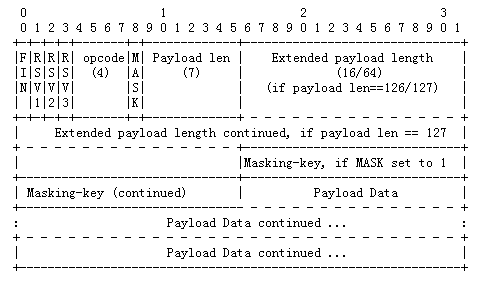
\includegraphics {frame.png}
    \end {figure}

    \begin {itemize}
    \item {FIN:1位}\par
          {表示这是消息的最后一帧(结束帧), 一个消息由一个或多个数据帧构成. 若消息由一帧构成, 起始帧即结束帧.}\par

    \item {RSV1, RSV2, RSV3:各1位}\par
          {MUST be 0 unless an extension is negotiated that defines meanings for non-zero values. If a nonzero value is received and none of the negotiated extensions defines the meaning of such a nonzero value,  the receiving endpoint MUST Fail the WebSocket Connection.}\par
          {如果未定义扩展, 各位是0;如果定义了扩展, 即为非0值. 如果接收的帧此处非0, 扩展中却没有该值的定义, 那么关闭连接.}\par

    \item {OPCODE:4位}\par
          {解释PayloadData, 如果接收到未知的opcode, 接收端必须关闭连接.}\par
          {0x0表示附加数据帧}\par
          {0x1表示文本数据帧}\par
          {0x2表示二进制数据帧}\par
          {0x3-7暂时无定义, 为以后的非控制帧保留}\par
          {0x8表示连接关闭}\par
          {0x9表示ping}\par
          {0xA表示pong}\par
          {0xB-F暂时无定义, 为以后的控制帧保留}\par

    \item {MASK:1位}\par
          {用于标识PayloadData是否经过掩码处理. 如果是1, Masking-key域的数据即是掩码密钥, 用于解码PayloadData. 客户端发出的数据帧需要进行掩码处理, 所以此位是1.}\par

    \item {Payload length:7位, 7+16位, 7+64位,  PayloadData的长度(以字节为单位)}\par
          {如果其值在0-125, 则是payload的真实长度.}\par
          {如果值是126, 则后面2个字节形成的16位无符号整型数的值是payload的真实长度. 注意, 网络字节序, 需要转换.}\par
          {如果值是127, 则后面8个字节形成的64位无符号整型数的值是payload的真实长度. 注意, 网络字节序, 需要转换.}\par
          {长度表示遵循一个原则, 用最少的字节表示长度(我理解是尽量减少不必要的传输). 举例说, payload真实长度是124, 在0-125之间, 必须用前7位表示;不允许长度1是126或127, 然后长度2是124, 这样违反原则.}\par

    \item {分片: 这种情况就比较复杂, 具体可以参考rfc, 一般在日常中用到的应该会比较少.}\par
    \end {itemize}
}

\section {\ZHH 客户端API} {
    {WebSocket的客户端API可以参考\href{http://www.tutorialspoint.com/html5/html5_websocket.htm}{Tutorial},  一个简单的代码参考: }\par
\begin{lstlisting}[language=html]
<!DOCTYPE HTML>
<html>
<head>
    <script type="text/javascript">
    function WebSocketTest()
    {
        if ("WebSocket" in window)
        {
            alert("WebSocket is supported by your Browser!");
            // Let us open a web socket
            var ws = new WebSocket("ws://localhost:9998/echo");
            ws.onopen = function()
            {
                // Web Socket is connected,  send data using send()
                ws.send("Message to send");
                alert("Message is sent...");
            };
            ws.onmessage = function (evt)
            {
                var received_msg = evt.data;
                alert("Message is received...");
            };
            ws.onclose = function()
            {
                // websocket is closed.
                alert("Connection is closed...");
            };
        }
        else
        {
            // The browser doesn't support WebSocket
            alert("WebSocket NOT supported by your Browser!");
        }
    }
    </script>
</head>
<body>
    <div id="sse">
        <a href="javascript:WebSocketTest()">Run WebSocket</a>
    </div>
</body>
</html>
\end{lstlisting}
}

\section {\ZHH WebSocket服务器} {
    {目前开源的WebSocket server的代码还是不少的.}\par
    {自己也整理过一份C的, 支持上面三种握手情况, 并嵌在reactor框架下, 使用chrome测试过: \href{https://github.com/gaccob/gbase/blob/master/net/wsconn.h}{gbase-wsconn}}\par
    {目前主流的浏览器对WebSocket的支持: }\par
\begin {table} [htbp]
    \centering
    \begin {tabular} {| c | c |}
        \hline
        Chrome  &   Supported in version 4+ \\
        \hline
        Firefox &   Supported in version 4+ \\
        \hline
        Internet Explorer &  Supported in version 10+ \\
        \hline
        Opera &  Supported in version 10+ \\
        \hline
        Safari &  Supported in version 5+ \\
        \hline
    \end{tabular}
\end {table}
}

\section {\ZHH 参考文章} {
    {1. \href{http://zh.wikipedia.org/wiki/WebSocket}{WIKI}}\par
    {2. \href{http://www.ibm.com/developerworks/cn/web/1112_huangxa_websocket/}{使用 HTML5 WebSocket 构建实时 Web 应用}}\par
    {3. \href{http://blog.csdn.net/fenglibing/article/details/7100070}{WebSocket不同版本的三种握手方式以及一个Netty实现JAVA类}}\par
    {4. \href{http://www.cnblogs.com/caosiyang/archive/2012/08/14/2637721.html}{WebSocket协议分析}}\par
}

\end{document}

